\thispagestyle{empty}
\begin{center}
	\vspace{\stretch{0.7}}
	{\Huge Wonsole} \\
	\medskip
	{\LARGE The new web console for power users} \\ 
	\bigskip
	{\Huge User Manual} \\ 
	\vspace{\stretch{0.3}}
	
\includegraphics[width=2.5in]{image/logo-ntnu.pdf} \\
	
\includegraphics[width=2.5in]{image/logo-netlight.png}
\end{center}
{\Large \textsc{Customer Driven Project}} \\
{\large \today \\Team: Ivo Dlouhy, Martin Havig, Øystein Heimark, Oddvar Hungnes}
\newpage

\setcounter{tocdepth}{1}
\tableofcontents
\clearpage
\listoffigures


\chapter{Introduction}
This document describes how to use the Wonsole application. It contains a user
tutorial as well as command refence.

\chapter{Basics}
User interface for wonsole is minimal a simple, so that the funcionality gets
presented in a clear way. If you see the main screen in the
picture \ref{wonsole2-00}, on the left hand side, there is a GUI - Graphical
User Interface - this is where data get presented as graphics. On the right hand side, there is a console window. This is a place
where user can input the commands and send the commands to the system by
pressing enter.

By default the list of available databases is displayed in GUI and
command prompt in console.


\begin{figure}
\centering
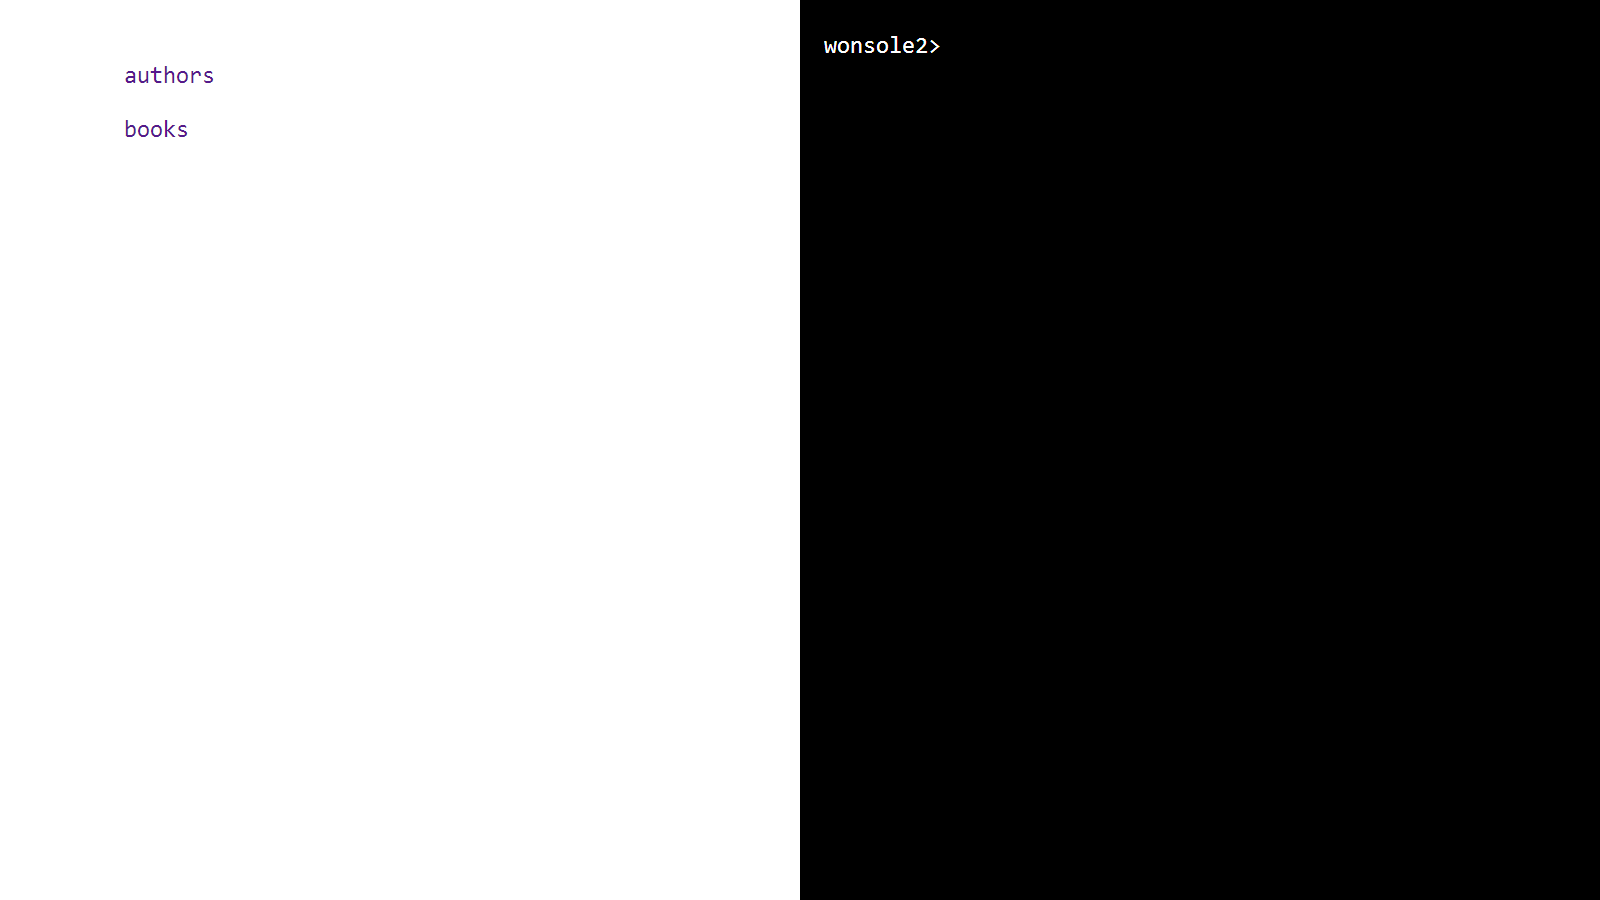
\includegraphics[width=\textwidth]{../../manual/screenshot/wonsole2/wonsole2-00.png}
\caption{Main screen}
\label{wonsole2-00}
\end{figure}

\chapter{Tutorial}

\section{Database: db}
The most basic command in Wonsole is the command to open, or switch database. It
has this format:
\begin{verbatim}
db DATABASE
\end{verbatim}
Where DATABASE is the name of the database to open. Databases are listed in GUI
and they can be opened by clicking at the name too.

After issuing the command, the database contents are displayed in GUI, see
picture \ref{wonsole2-02}.
Wonsole uses document oriented database, so it is list of documents indexed by numbers.
From each document the title attribute is displayed as preview.


\begin{figure}
\centering
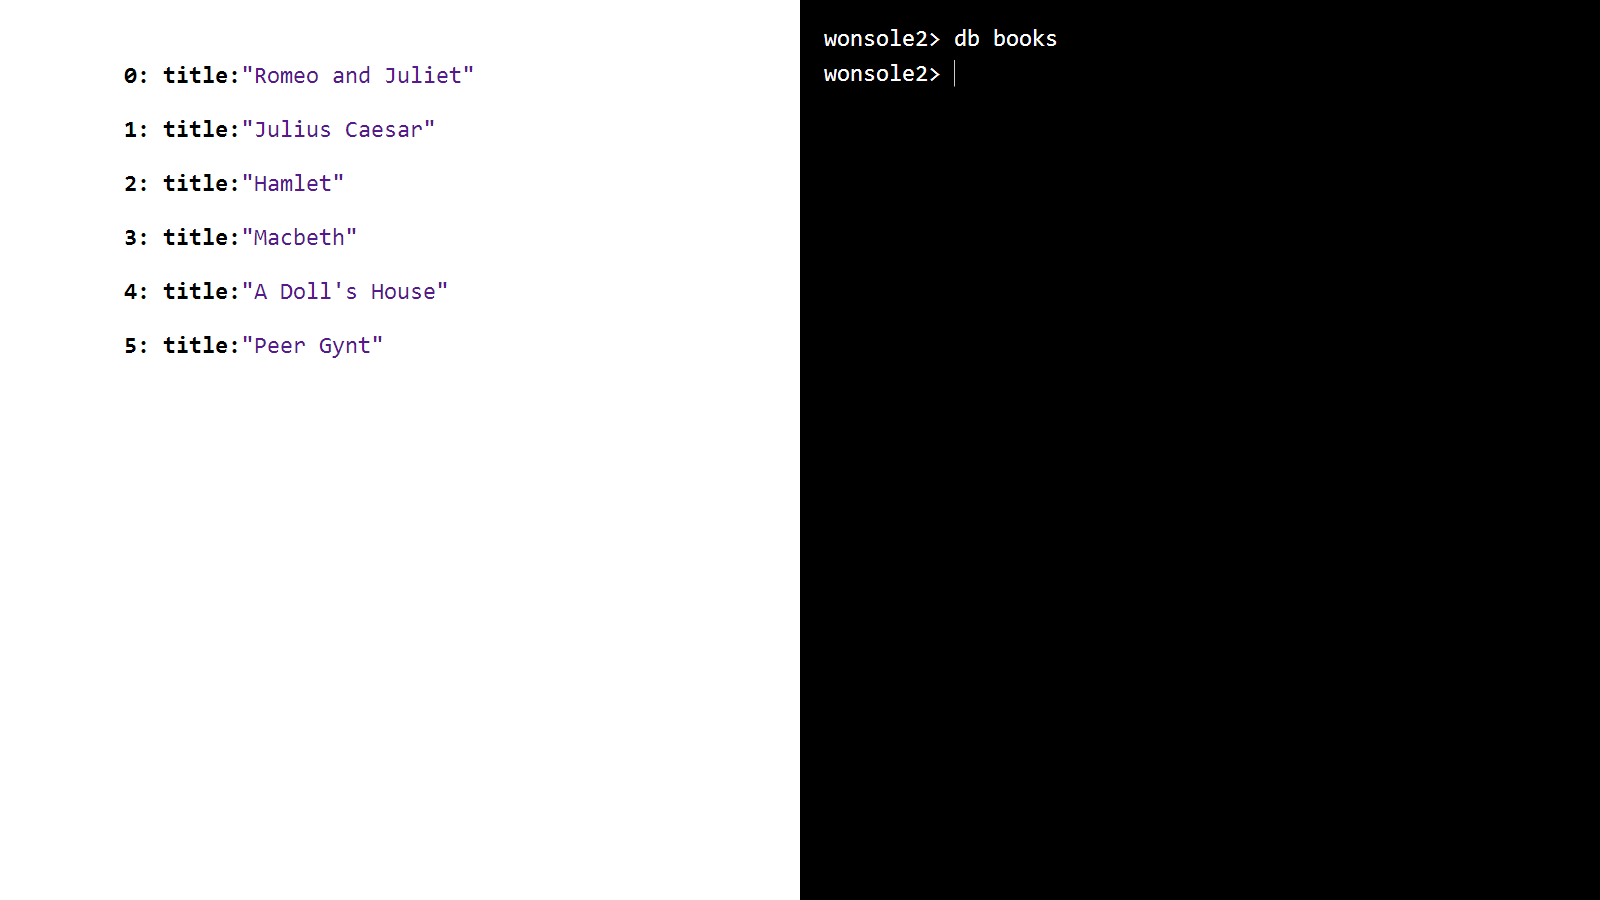
\includegraphics[width=\textwidth]{../../manual/screenshot/wonsole2/wonsole2-02.png}
\caption{Database open}
\label{wonsole2-02}
\end{figure}

Same command can be used to switch the database anywhere in the workflow as in
picture \ref{wonsole2-04}.

\textit{Note: All uncommited changes are lost when switching the database.}

\begin{figure}
\centering
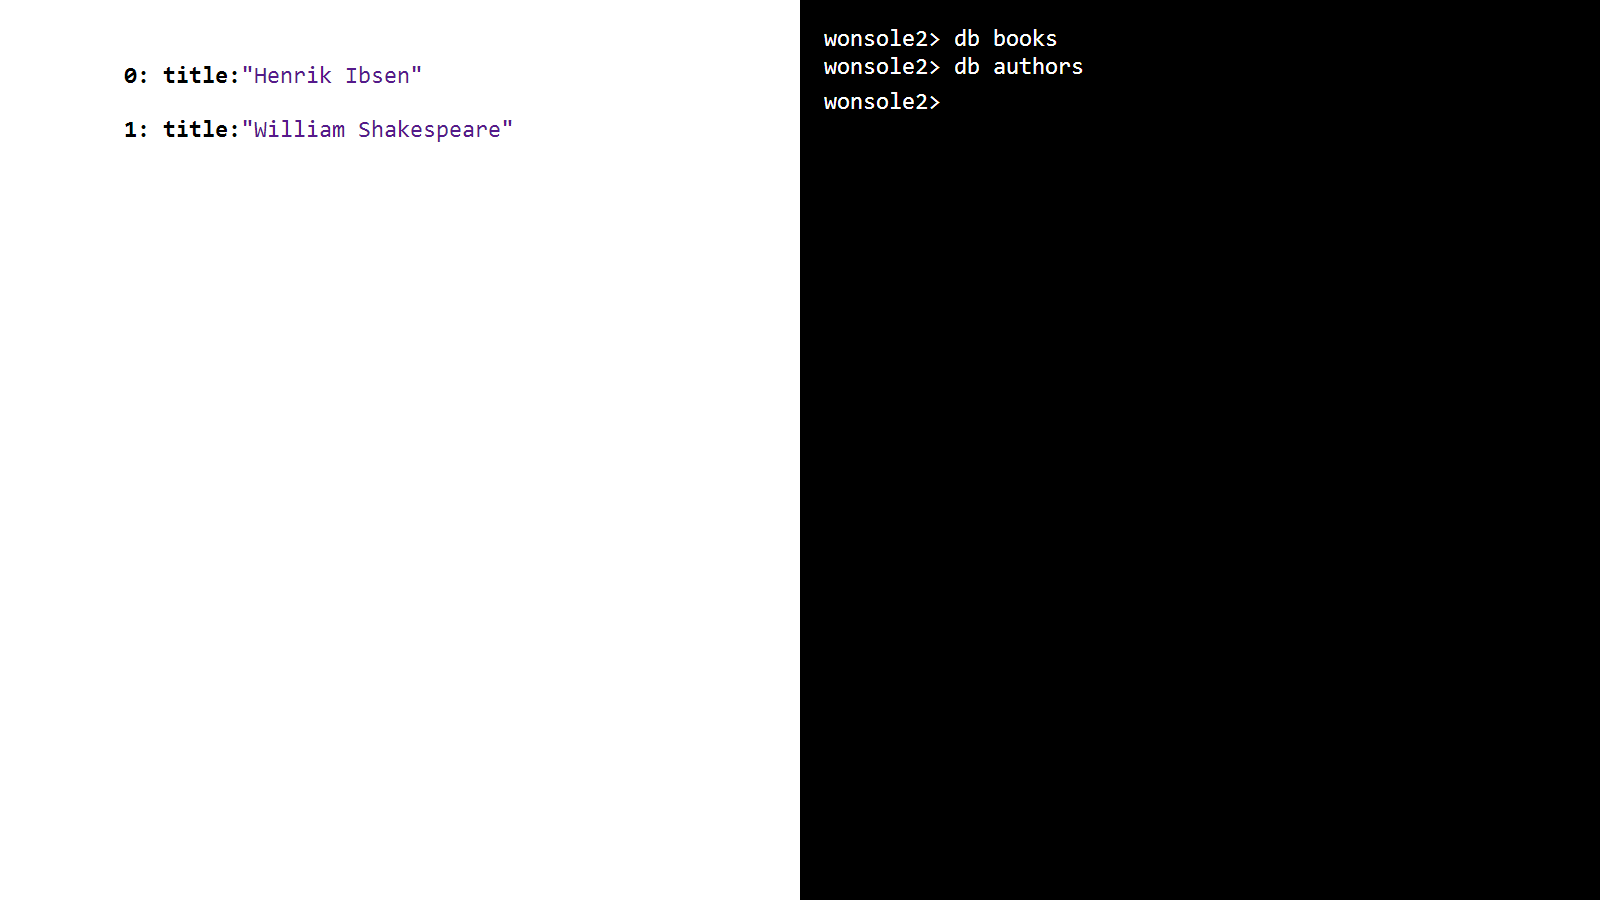
\includegraphics[width=\textwidth]{../../manual/screenshot/wonsole2/wonsole2-04.png}
\caption{Database switch}
\label{wonsole2-04}
\end{figure}

\section{Presentation: print and view}
Command print is available to display data in plaintext instead of using GUI.
It's syntax is very simple - it has one attribute: variable or data to print.
\begin{verbatim}
print DATA
\end{verbatim}
Command loads the data, converts it into text and prints in the console as ssen
in picture \ref{wonsole2-10}.

\begin{figure}
\centering
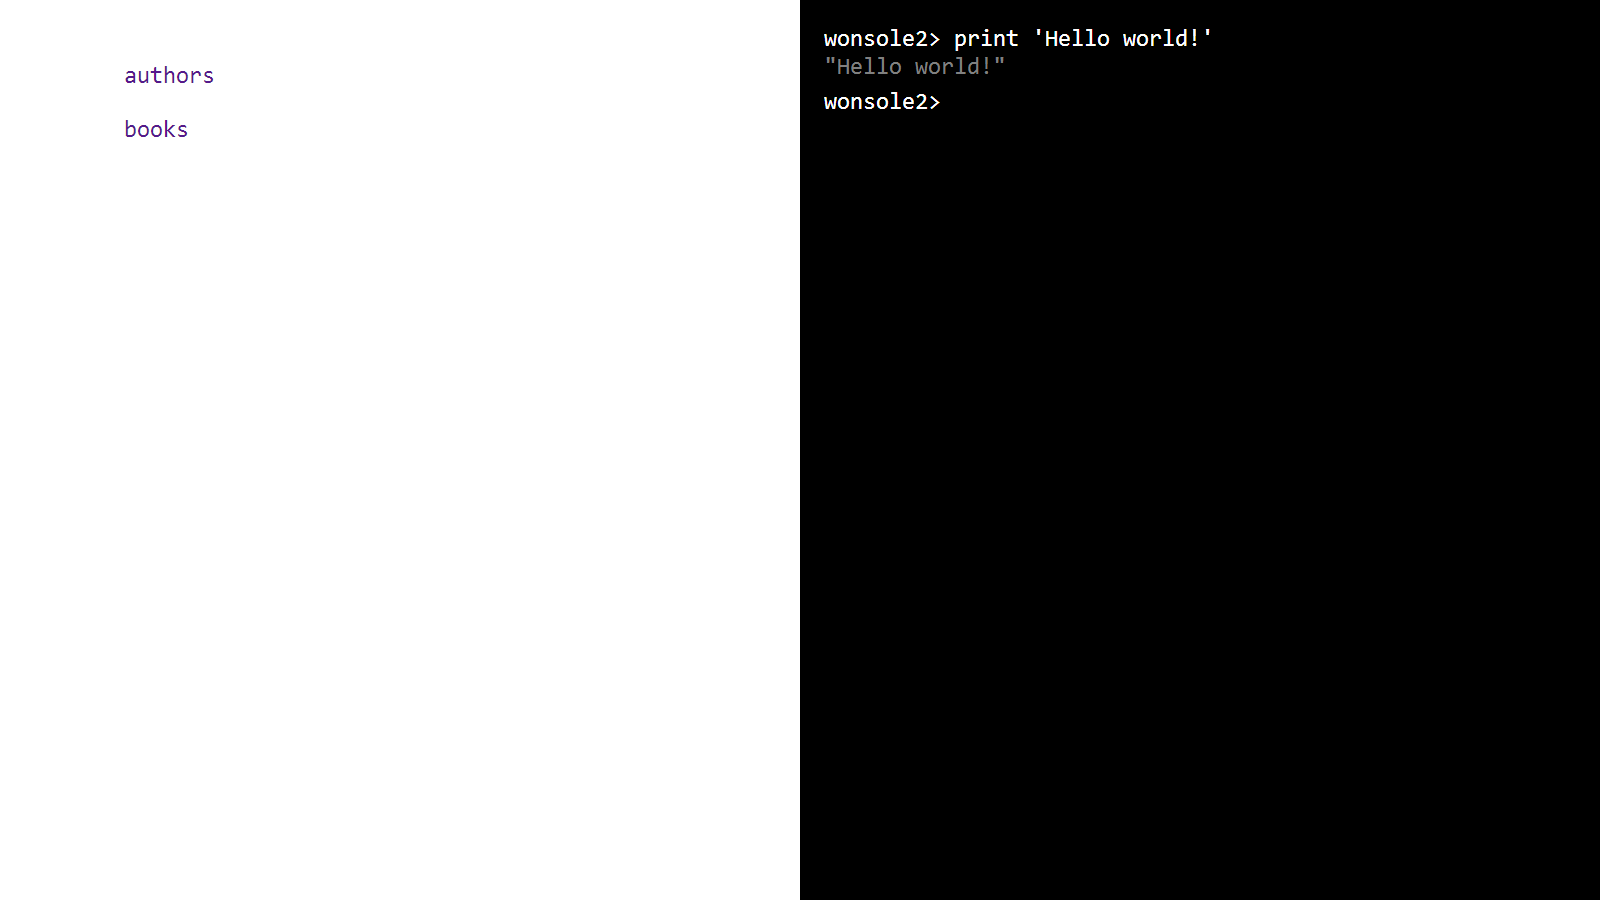
\includegraphics[width=\textwidth]{../../manual/screenshot/wonsole2/wonsole2-10.png}
\caption{Print}
\label{wonsole2-10}
\end{figure}

Oposite of the print command there is view. It displays the complex variable in
the GUI.
\begin{verbatim}
view VARIABLE
\end{verbatim}

\section{JavaScript integration}
Wonsole includes complete JavaScript language to the command set. If user issues
acommand, that is not recognized as the Wonsole command, this input gets
evaluated as JavaScript. You can for example issue a helper command, that does
some required functionality not supported by Wonsole and than continue using
default Wonsole commands, JavaScript language is 100% integrated into Wonsole.

\begin{verbatim}
var new = "New variable" //Javascript
print variable
"New variable"
\end{verbatim}

This is an example of creating a new JavaScript variable and using it in simple
Wonsole command, demonstration on picture \ref{wonsole2-15}.

\textit{Note: This is advanced functionality. JavaScript language is very
complex and it is the user full responsibility to use it in a safe, suitable
way.}
 

\begin{figure}
\centering
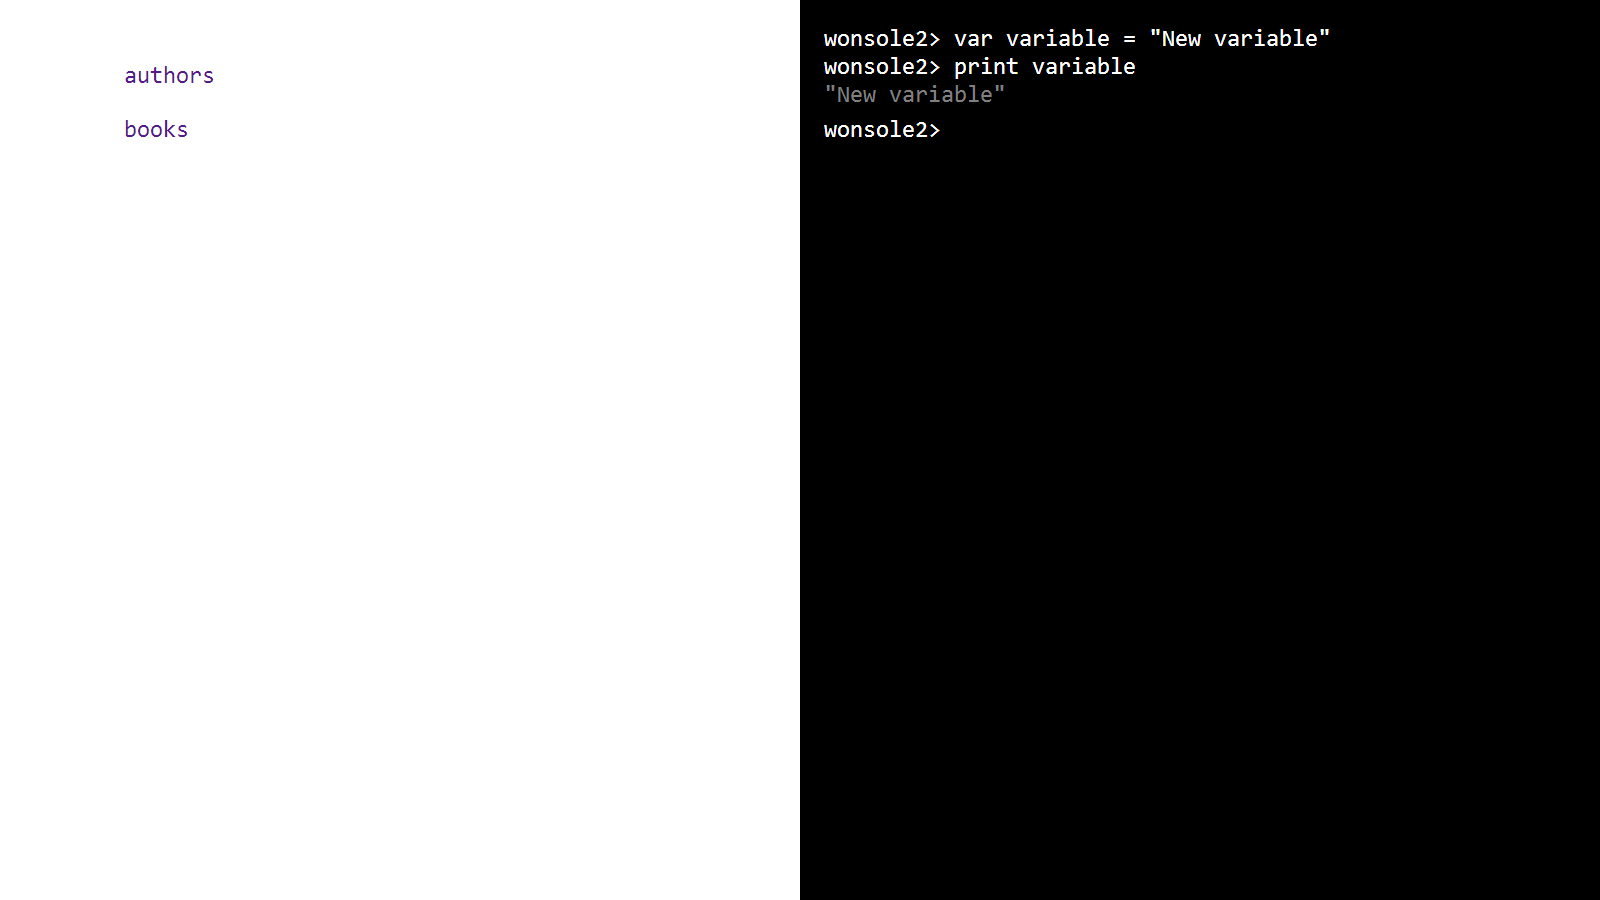
\includegraphics[width=\textwidth]{../../manual/screenshot/wonsole2/wonsole2-15.png}
\caption{Javascript integration}
\label{wonsole2-15}
\end{figure}

\section{Display: Quiet}
When Wonsole displays a list of documents saved in the database (see command
db) by default it uses quiet mode. In quiet mode, it displays only object index and
value of the title attribute as a object identification as you can see in
picture \ref{wonsole2-18}.

\begin{figure}
\centering
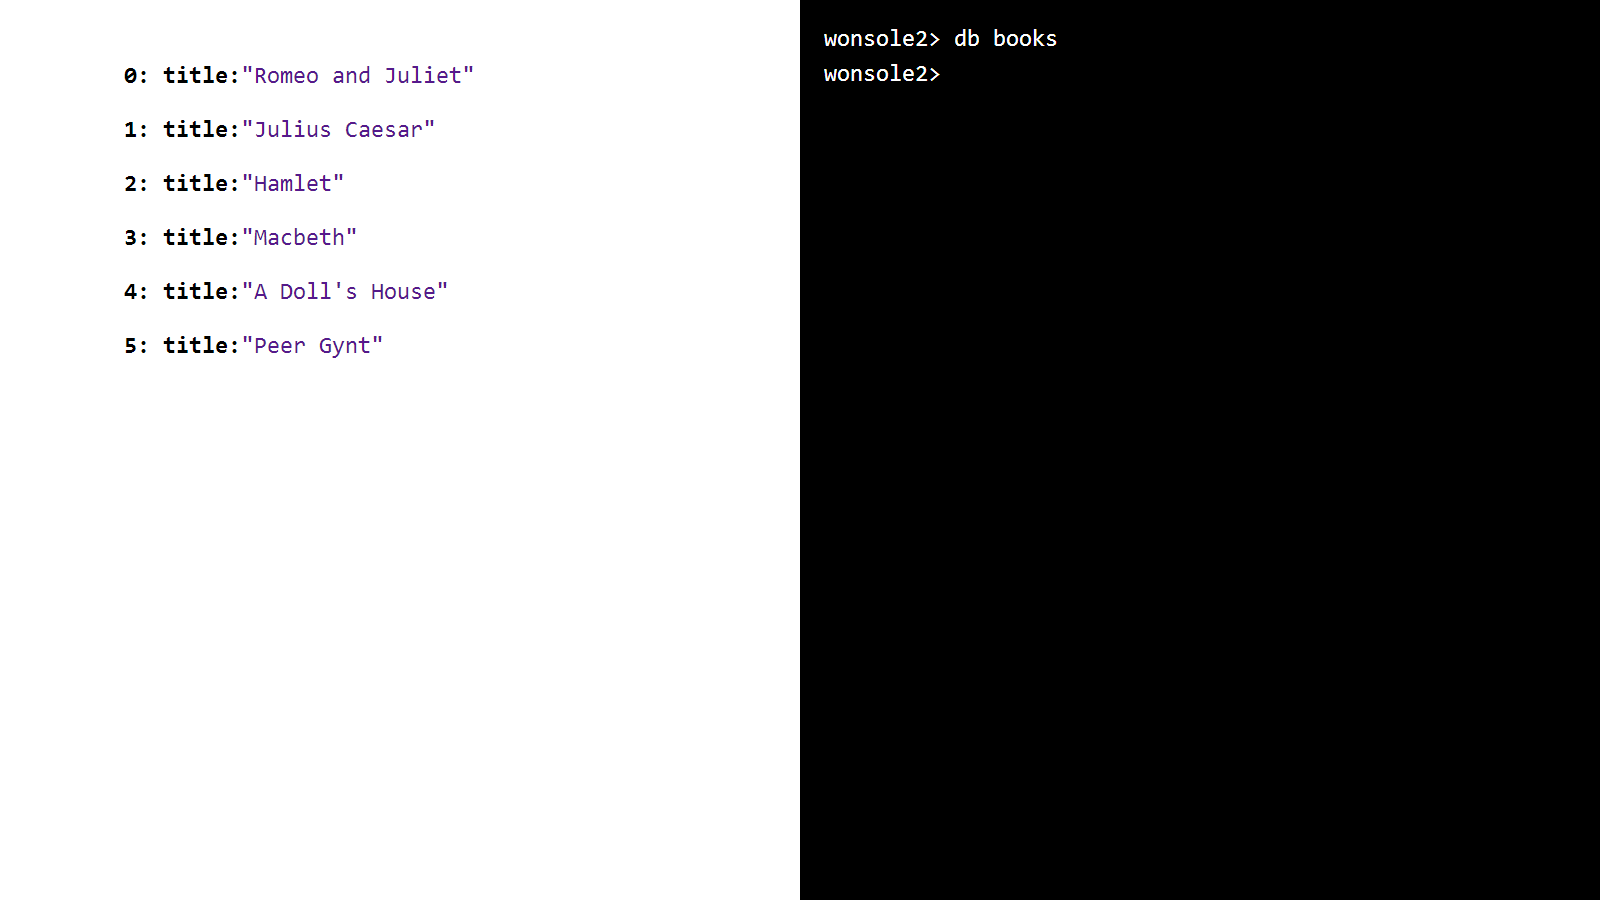
\includegraphics[width=\textwidth]{../../manual/screenshot/wonsole2/wonsole2-18.png}
\caption{Quiet mode on}
\label{wonsole2-18}
\end{figure}

\begin{verbatim}
quiet
\end{verbatim}

You can toggle preview mode by using command quiet. When toggled off, all
attributes of the object are displayed - but only the simple data types. If the
atribute is complex, the Object keyword is displayed instead, see picture
\ref{wonsole2-20}.

\begin{figure}
\centering
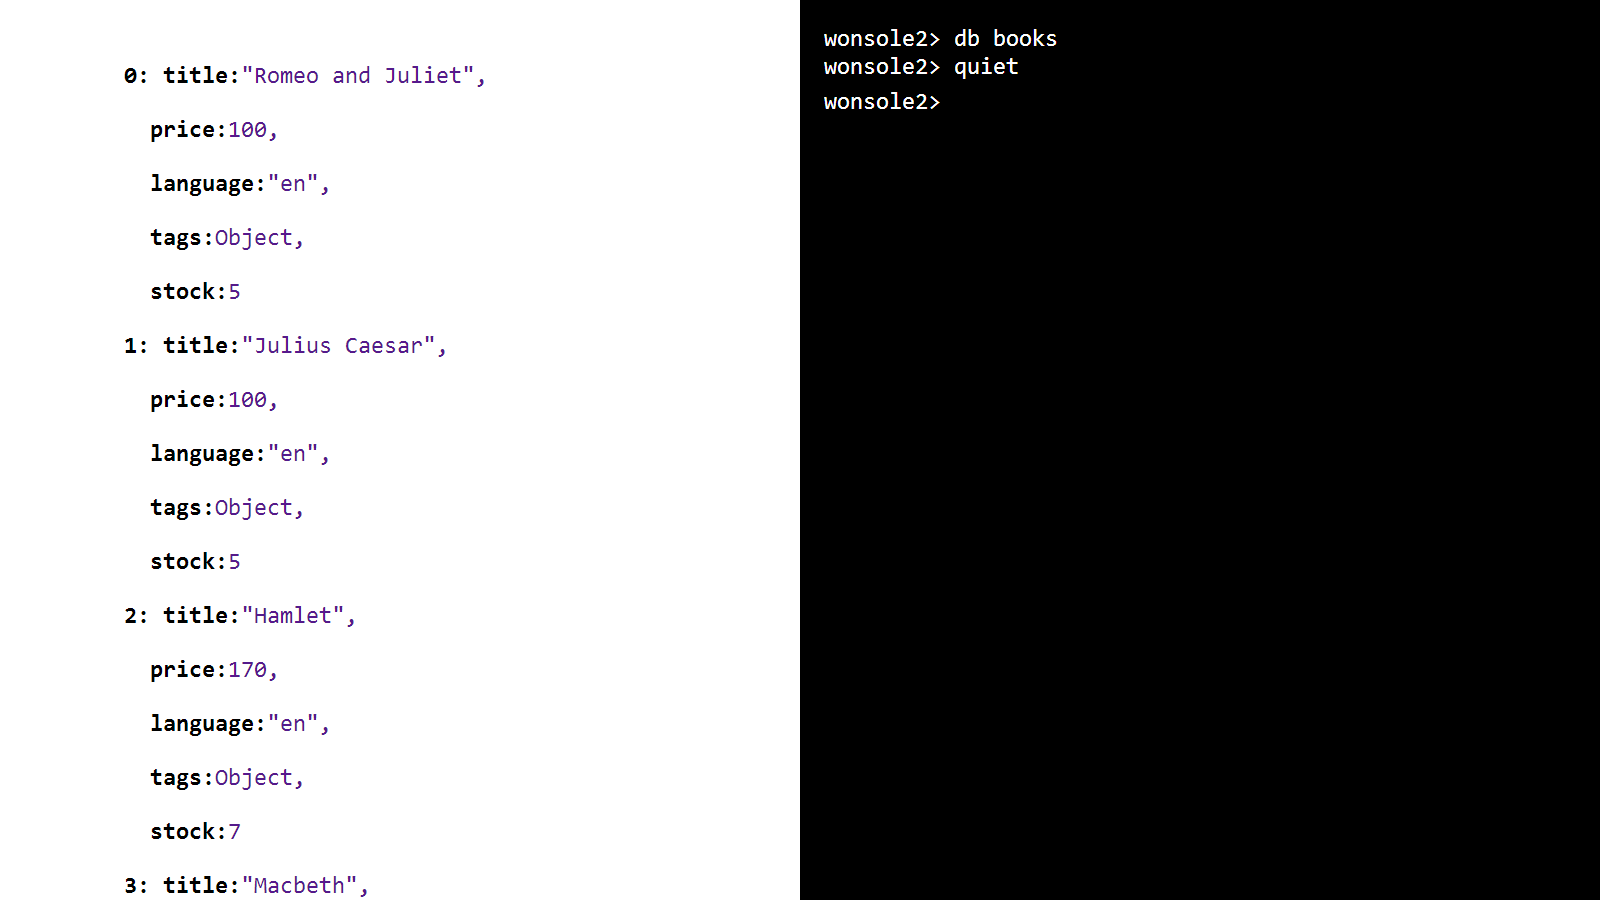
\includegraphics[width=\textwidth]{../../manual/screenshot/wonsole2/wonsole2-20.png}
\caption{Quiet mode off}
\label{wonsole2-20}
\end{figure}


\section{Documents: docs and doc}
After opening the database, list of documents is loaded. Is is stored in
\verb|docs| variable for you to work with. This variable is an array, so you can
index it and get a single document object as seen in picture \ref{wonsole2-26}.

\begin{verbatim}
db books
docs
[...]
\end{verbatim}
 

\begin{figure}
\centering
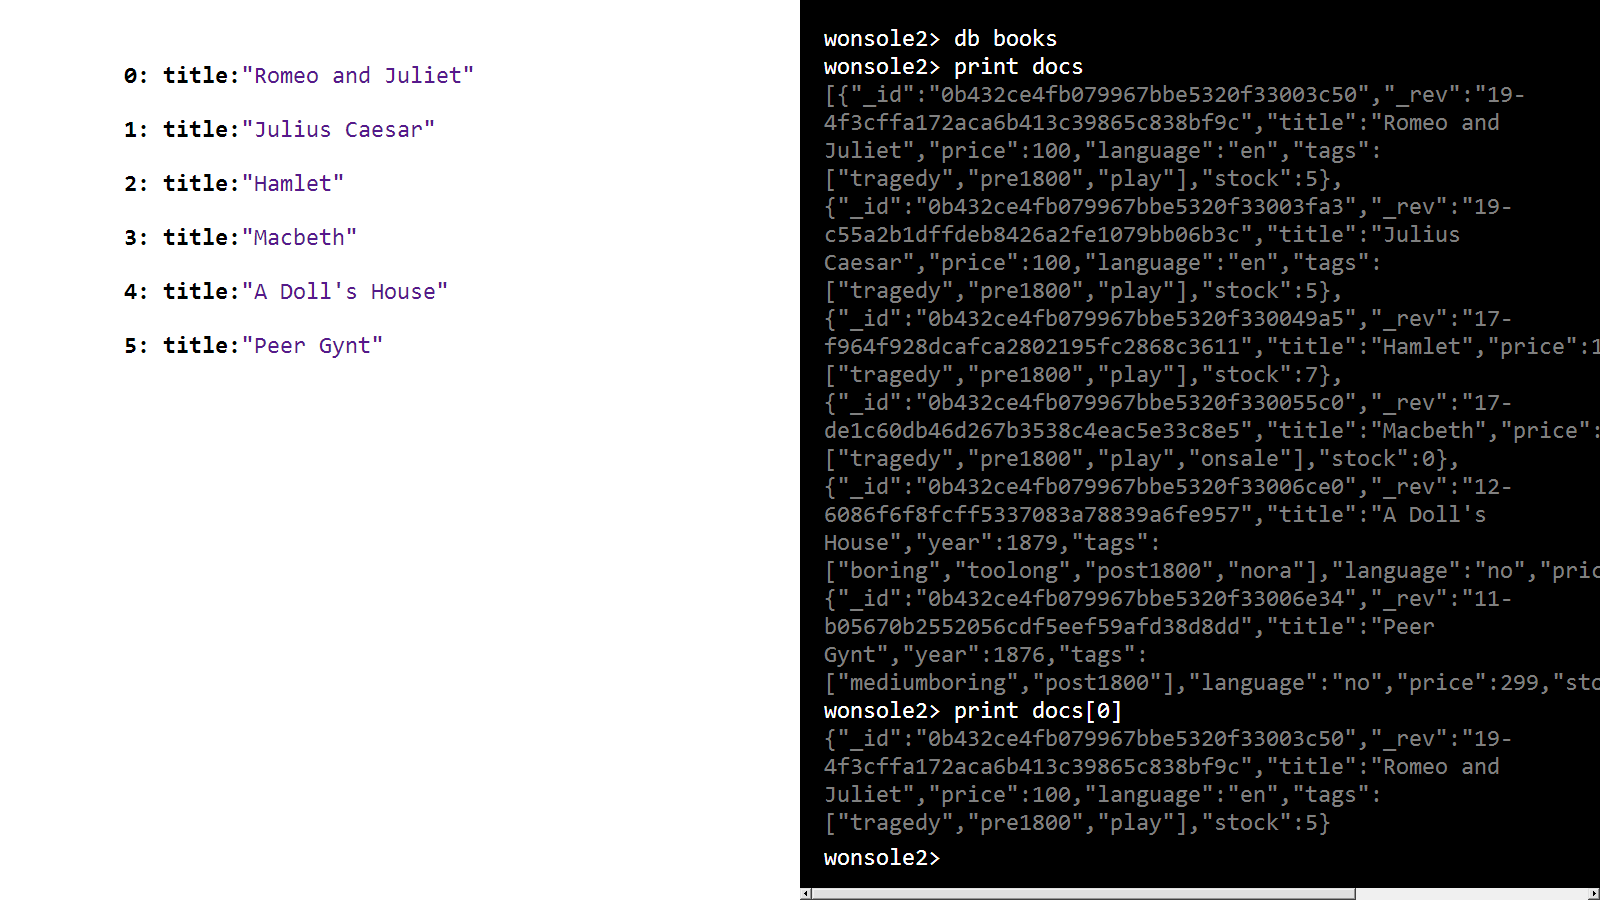
\includegraphics[width=\textwidth]{../../manual/screenshot/wonsole2/wonsole2-26.png}
\caption{List of documents}
\label{wonsole2-26}
\end{figure}

Documents displayed in the document list mode are indexed using numbers. You can
use these numbers together with \verb|doc| command to open a single document.
This command can be also used to switch between documents, you just have to
issue it with different index. The opened document is stored inside a \verb|doc|
variable as demonstrated in picture \ref{wonsole2-32}.

\begin{figure}
\centering
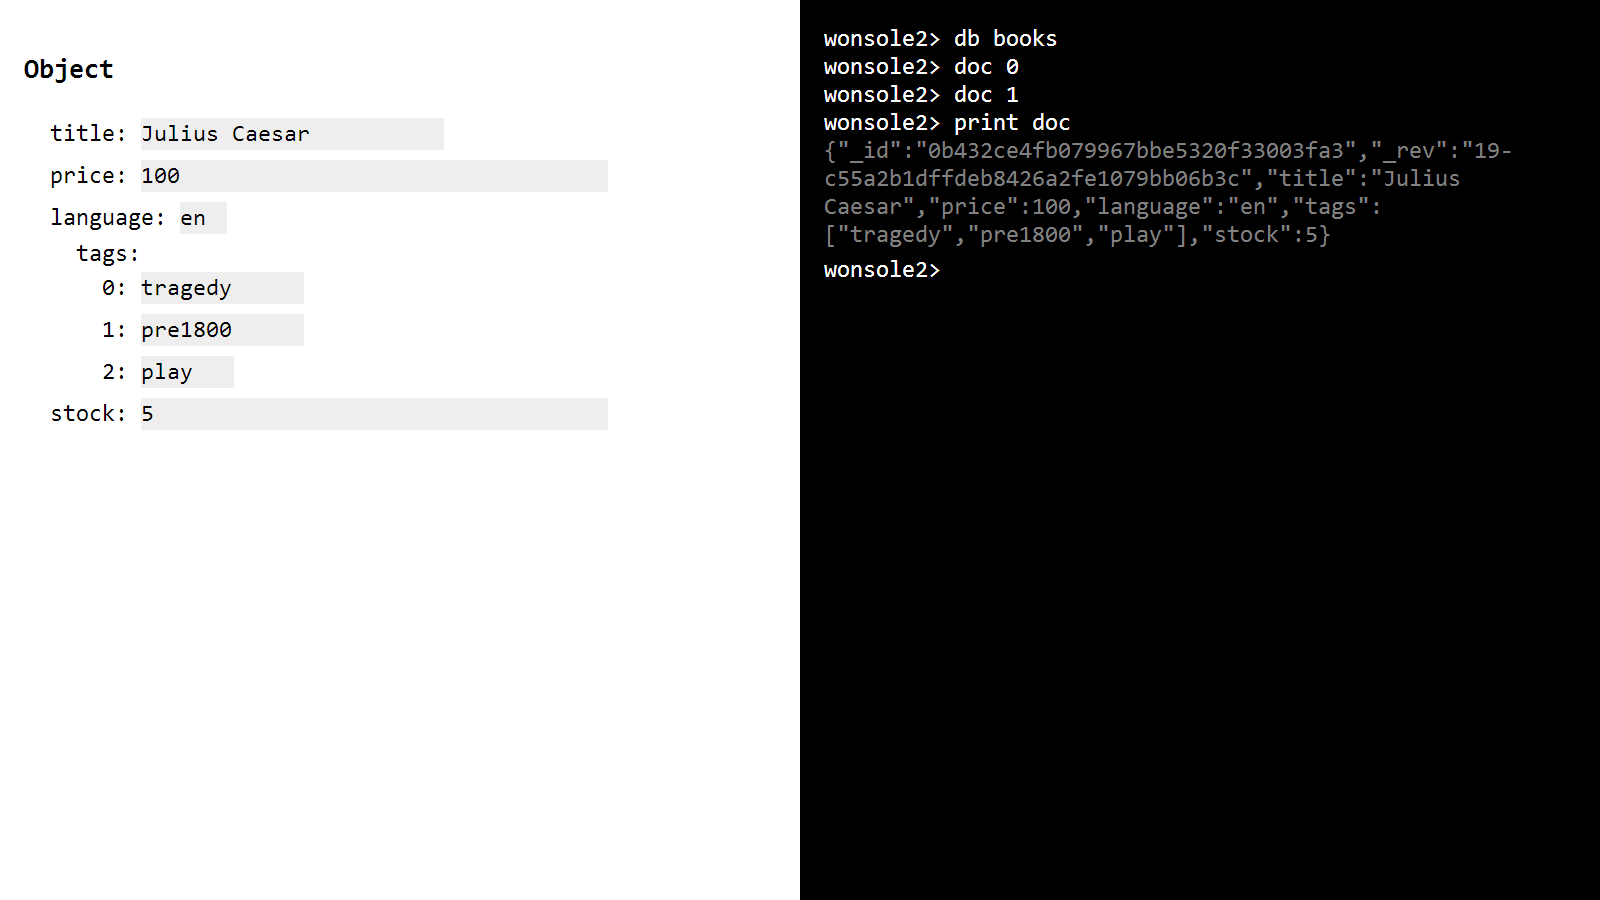
\includegraphics[width=\textwidth]{../../manual/screenshot/wonsole2/wonsole2-32.png}
\caption{Doc object}
\label{wonsole2-32}
\end{figure}

To change the document, use a simple assignment command. This way you can modify
the object freely, you can also add a new attribute. Example is in the picture
\ref{wonsole2-38}


\begin{figure}
\centering
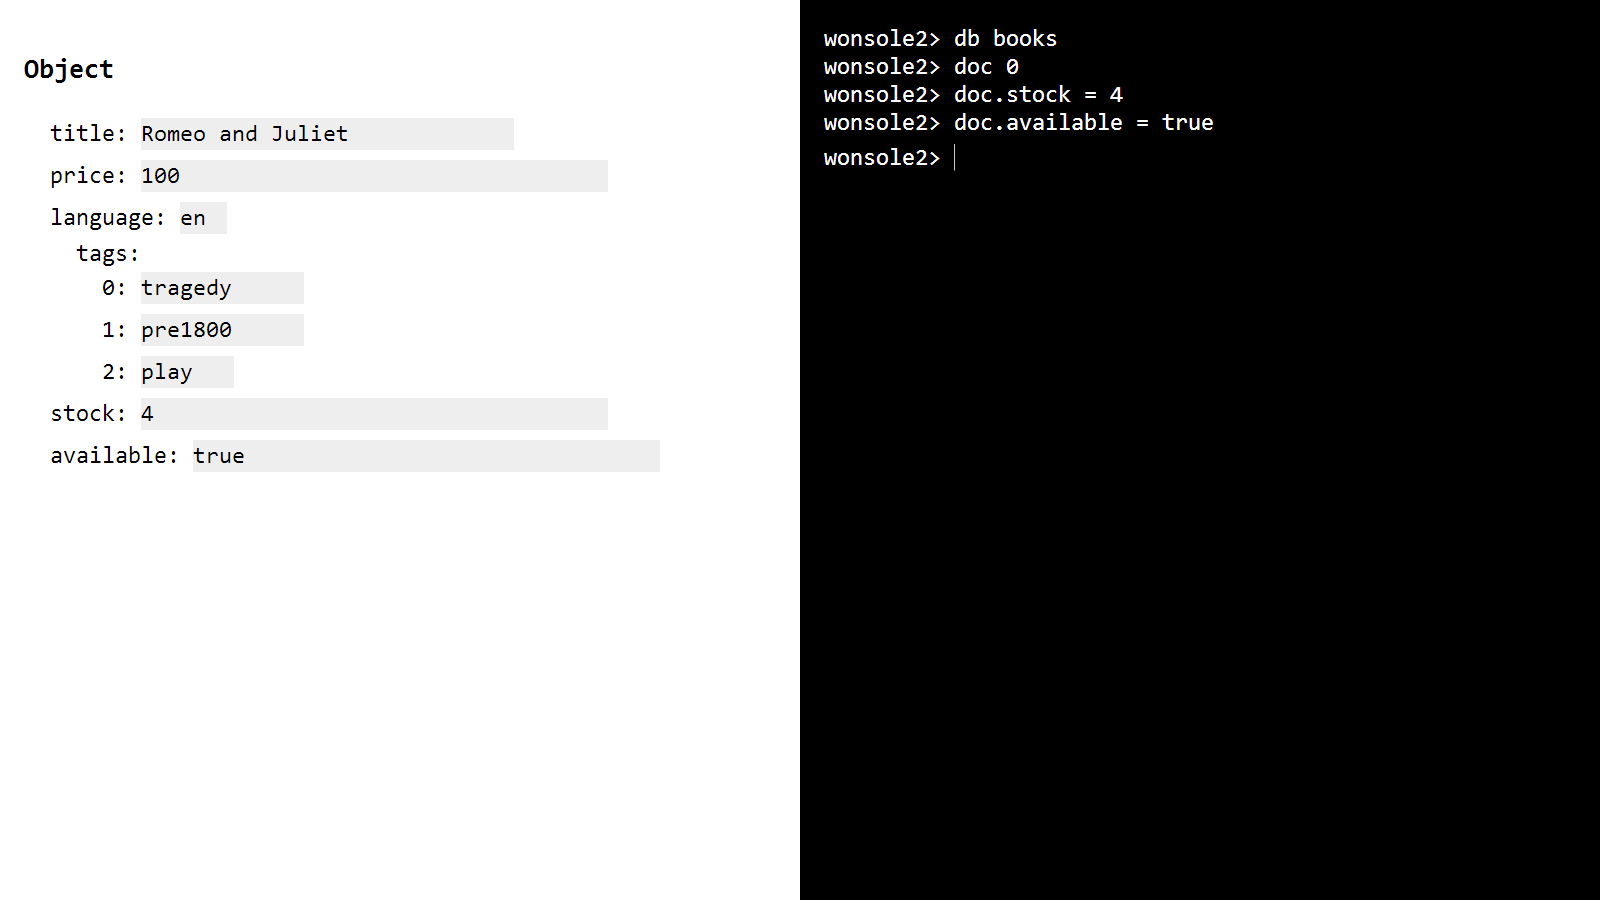
\includegraphics[width=\textwidth]{../../manual/screenshot/wonsole2/wonsole2-38.png}
\caption{Modification of doc}
\label{wonsole2-38}
\end{figure}



\section{Transactions: Commit and Rollback}
All changes you perform on objects are local, so at any point during the
modification process, transaction, you have a option to save all the changes to
database using command \verb|commit| or to throw away all local changes and load
back the values from database with command \verb|rollback|. This functionality
can be used as an undo command, it is up to you, how often you commit the
changes.


\section{Objects: Add and Remove}
To add a new object, use an \verb|add| command. It has one parameter, object to
add. If you are not sure, just create an empty object. Otherwise you can
directly define specific object attributes as in picture \ref{wonsole2-48}. The
new object will immediatelly appear in document list, so you can open
it and continue working with it, for example add a new attribute as in picture
\ref{wonsole2-48}.


\begin{figure}
\centering
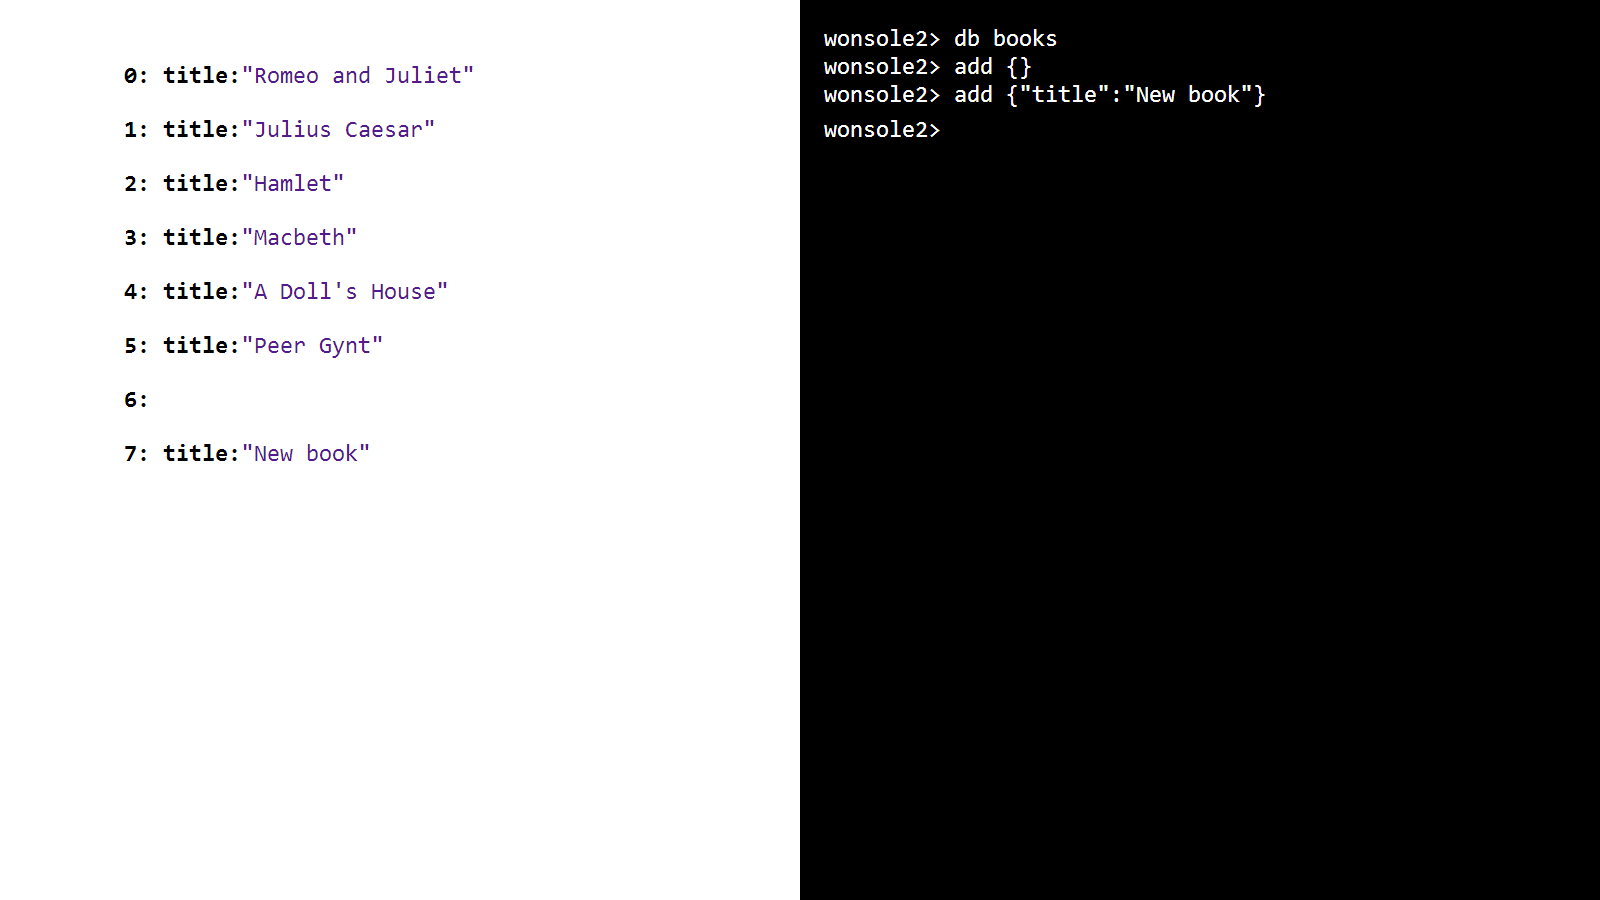
\includegraphics[width=\textwidth]{../../manual/screenshot/wonsole2/wonsole2-48.png}
\caption{Add}
\label{wonsole2-48}
\end{figure}

\begin{figure}
\centering
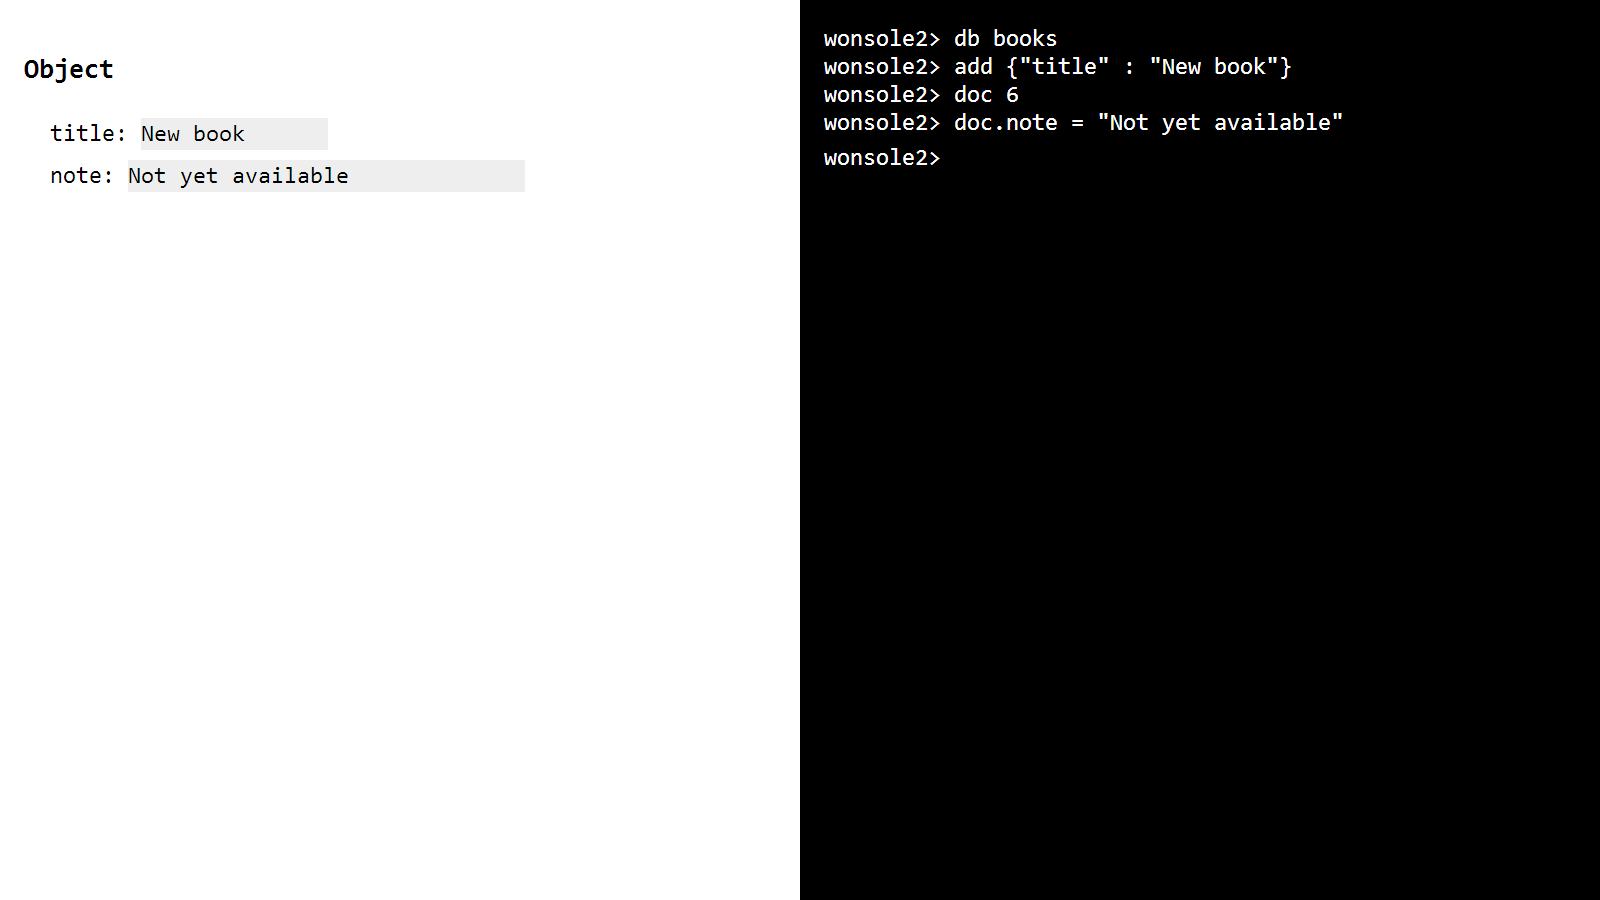
\includegraphics[width=\textwidth]{../../manual/screenshot/wonsole2/wonsole2-55.png}
\caption{Add and modify}
\label{wonsole2-55}
\end{figure}
